\documentclass[a4paper]{jpconf}
\usepackage{amsmath}
\usepackage{amssymb}
\usepackage{cite}
\usepackage{changepage}
\usepackage{graphicx}
%\usepackage{float}
%% \usepackage[square,sort&compress]{natbib}
\bibliographystyle{iopart-num}

\begin{document}
\title{Top Quark Partner Spectra}
\author{2025061L}
\address{School of Physics \& Astronomy, University of Glasgow, UK}
\ead{2025061L@student.gla.ac.uk}
\begin{abstract}
One possible extension to the Standard Model considers the Higgs boson as a composite state of some strongly interacting sector. This scenario does not exhibit the allegedly unattractive feature of a large fine-tuning. We consider the Higgs as a pseudo-Nambu-Goldstone boson which arises from a spontaneous symmetry breaking \(SO(5) \to SO(4)\). Massive fermionic resonances are described using partial compositeness, and a mass matrix is constructed describing such resonances for the top quark. We employ a bi-unitary transformation (quark basis change) using the singular value decomposition technique to deduce the mass of top partners. This is performed over a range of energy scales and we find that solutions exist for each. Furthermore, the resulting top partner masses exhibit values within reach of the Large Hadron Collider. We conclude that this model is viable and testable in the near future.      
\end{abstract}
\section{Introduction}
The discovery of a Higgs-like boson \cite{cmsHiggs, atlasHiggs} at the Large Hadron Collider (LHC), CERN, was the crowning of an international effort in science and engineering that spanned over 40 years. Efforts are ongoing to confirm if this particle is the Standard Model (SM) Higgs, and thus completing perhaps the most successful theory in all of science, or that of some other theoretical regime. \\
\hfill\break
The Higgs mechanism, proposed in the 1960s by Higgs \cite{higgs}, Brout and Englert \cite{englert_brout} and many others, is essential in describing the mass generation of gauge bosons. It introduces a complex scalar field, the Higgs field, with a non-zero vacuum expectation value. As a consequence, the electroweak symmetry is spontaneously broken to the electromagnetic symmetry. Simultaneously, three of the four degrees of freedom of the Higgs field are absorbed by the \(W^\pm\) and \(Z\) vector bosons to acquire masses. This phenomenon is called electroweak symmetry breaking (EWSB). Fermions also acquire mass in a consistent but distinct manner - through a Yukawa interaction with the field and its conjugate. The remaining degree of freedom corresponds to a scalar particle, the Higgs boson \cite{djouadi}. There are many alternate theories that hold a Higgs as the root of EWSB, but offer more natural solutions to issues such as the Hierarchy problem. \\
\hfill\break
The Hierarchy problem, in somewhat loose terms, asks a simple question: why is the Higgs mass 125 GeV? Or more specifically, why is it so much lighter than the Planck scale \(\sim10^{19}\)GeV? When virtual particle-antiparticle pairs appear in the vacuum, their interaction with the Higgs is expected to make a contribution to the Higgs-boson squared mass \(m_{H}^2\). An analogy is made by Guidice \cite{guidice}: \\
\begin{adjustwidth}{1cm}{1cm}
\emph{Let us replace the quantum fluctuations of the vacuum with the more familiar thermal fluctuations of a thermodynamic system of a large number of particles at a temperature T. The particles (which I will call P) in this thermal bath play the role of the virtual particles in the quantum vacuum, and T the role of the maximum available energy Λ. Let us now insert inside the box containing this hot P-particle gas a different particle initially at rest. I will call it H, as it plays the role of the Higgs in my analogy. At some initial time, H has zero velocity and therefore its energy is equal to its mass, which I take it to be much smaller than the temperature (\(E_{H} = m_{H} \ll T\)). However, by statistical-mechanics arguments, we expect that the collisions of the particles P will soon bring H in thermal equilibrium, and therefore its energy will quickly become of order T. This is very similar to what happens in the quantum system...} \\
\end{adjustwidth}
\hfill\break
\noindent The exact expressions for these quantum corrections are gained from taking the path integral around the loops of such diagrams shown in Fig. \ref{fig:feyn}. Since the virtual particle momenta can take any value up to infinity, the integral diverges and hence acts to drive the mass to infinity. Choosing to cut the loop integral momenta at a scale \(\Lambda\), the difference between the physical Higgs squared mass and the bare mass \(\left(m_{H}^0\right)^2\) contained in the unrenormalised Lagrangian is most notably given by\cite{djouadi}:
\begin{equation}
\label{eq1}
m_H^2 = \left(m_{H}^0\right)^2  + \frac{3\Lambda^2}{8\pi^2 v^2 M_H^2}\left(4m_t^2 - m_H^2 - 2m_W^2 - m_Z^2\right)
\end{equation}
where \(v\), \(m_t\), \(m_W\) and \(m_Z\) denote the Higgs vacuum expectation value, top quark mass, W boson mass and Z boson mass respectively. Making the naive assumption that the SM is expected to hold up to at most the Planck scale (where gravitational effects will then definitely call for its successor), requires an incredible fine-tuning of parameters between the bare mass and the radiative corrections, down to around the 16th decimal place. This is one manifestation of the Hierarchy problem and although itself presents no mathematical inconsistency, is deeply unsettling and considered highly unnatural that physics on one scale should depend entirely on another. Quantum mechanics does not affect the trajectory of a golf ball. If this argument is reversed and we ask at which energy scale the SM can be considered natural (i.e. \(\delta m_H^2/m_H^2\) is of order unity), we find \(\Lambda \sim\) TeV. This is strong motivation that any new physics present should reveal itself around the TeV scale, and indeed partly motivated the construction of the LHC at these energies.

\begin{figure}[h]
	\centering
	\includegraphics[width=12cm]{feynman} 
	\caption{The largest radiative corrections originate from the Higgs boson, massive gauge bosons, and top quark loops. We see from Eq.~\eqref{eq1} that each of these is inextricably linked to the vacuum expectation value of the Higgs field.}
	\label{fig:feyn}
\end{figure}

\section{Theory}
One extension to the SM considers the Higgs as a composite bound state which arises from a new strongly interacting sector \cite{kaplan}. This paradigm, known as composite Higgs models (CHM), requires minimal or no fine-tuning as the Higgs is protected from one-loop quadratic divergences by approximate global symmetries \cite{lhr}. In most cases, the Higgs is considered as a pseudo-Nambu-Goldstone boson (pNGB) of a spontaneous symmetry breaking, and can exhibit a mass much lighter than other strong resonances \cite{contino}. This is similar to the pion in quantum chromodynamics (QCD)\cite{burgess}. \\
\hfill\break
QCD can be well approximated by taking the masses of the up and down quark, \(m_u\) and \(m_d\), as zero. The QCD Lagrangian then acquires a very useful symmetry, where the corresponding symmetry group obtained is \(G = SU_L(2) \times SU_R(2)\). This is a chiral symmetry treating left- and right- chiral fermions differently. \(G\) is spontaneously broken in the QCD ground state, however it is observed that the hadron (composite quark object) spectrum does obey a representation of the approximate symmetry of \emph{isopsin}: \(SU_I(2)\), which can be understood at the quark level to be a diagonal subgroup of \(G\) treating left- and right- chiral fermions as identical. Thus we have the spontaneous symmetry breaking \(SU_L(2) \times SU_R(2) \to SU_I(2)\). Goldstone's theorem \cite{goldstone} states that we expect to find exactly as many spinless, massless bosons in the spectrum as there are broken generators. \(SU(N)\) has \(N^2-1\) generators hence for this symmetry breaking pattern we expect to find \((3+3) - 3 = 3\) particles. Indeed, for QCD, the \(\pi^{\pm}\) and \(\pi^0\) particles have the required quantum numbers to act as the Nambu-Goldsonte bosons (NGBs). The reason the pions are not massless (hence denoted pNGBs) is because the original symmetry \(G\) is approximate. pNGBs are characteristically light in comparison to the rest of the spectrum, as seen with the pions. \\
\hfill\break
The idea of the Higgs as a pNGB has been heavily studied. The following phenomenology has emerged \cite{ltlh}: all SM particles originate as elementary fields, external to the new strong sector. The communication with the Higgs and the strong dynamics, and thus the generation of mass after EWSB, occurs through linear couplings of the elementary fields with suitable strong sector operators. At low energies, below the confinement scale, the linear couplings become mixing terms among the elementary SM particles and some heavy composite resonance. The physical states after diagonalisation possess a composite component, realising the paradigm of partial compositeness first proposed by Kaplan \cite{kaplan1}. Associated with the fermionic operators, massive fermionic resonances emerge from the strong sector. These heavier partners provide a very promising direct experimental manifestation of the composite Higgs scenario at the LHC. \\
\hfill\break
In the explicit model considered here, the symmetry group of the strongly interacting sector is given by \(SO(5)\), which is spontaneously broken down to \(SO(4)\) at a scale \(f\). This is motivated again when we consider Goldstone's theorem. The number of generators of \(SO(N)\) is \(N(N-1)/2\) hence we have \(10 - 6 = 4\) degrees of freedom, the exact number required to recover the Higgs doublet under \(SU(2)\), as in the SM. Further details can be found in \cite{hlet_comp}. We look at the `minimal' scenario, coined `MCHM5' in the literature when using the fundamental (\textbf{5}) representation of \(SO(5)\). In this regime, a Lagrangian can be constructed which gives rise to the following mass matrix, for the set of fermionic resonances associated with the top quark (note Eq.~\eqref{eq3} simply introduces some labels):
\begin{align}
\label{eq2}
 -\mathcal{L}_{m} &= 
\overline{\begin{pmatrix}
t_{L} \\ T_{L} \\ X^{2/3}_{L} \\ \tilde{T}_{L}
\end{pmatrix}}
\begin{pmatrix}
0 & \Delta_{L} & 0 & 0 \\
0 & M_{0} + \frac{fys^{2}}{2} & \frac{yfs^{2}}{2} & \frac{yfsc}{\sqrt{2}} \\
0 & \frac{yfs^{2}}{2} & M_{0} + \frac{fys^{2}}{2} & \frac{yfsc}{\sqrt{2}} \\
\Delta_{R} & \frac{yfsc}{\sqrt{2}} & \frac{fysc}{\sqrt{2}} & M_{0} + yfc^{2}
\end{pmatrix}
\begin{pmatrix}
t_{R} \\ T_{R} \\ X^{2/3}_{R} \\ \tilde{T}_{R}
\end{pmatrix} + h.c. \\
\label{eq3}
&= \left(\psi_{L}^{0}\right)^\dag M^{t} \psi_{R}^{0} + h.c.	
\end{align}
\(\Delta_{L,R}\) describe the degree of mixing between composite and elementary states, \(M_{0} = 4\pi f\) is the composite mass scale, the dimensionless parameter \(0 \leq y \leq 4\pi\) represents some coupling between composite and elementary states and \(s\) and \(c\) are dimensionless constants dependent on the weak scale \(v \sim\) 246 GeV. \(\left(\psi_{L}^0\right)^\dag\) and \(\psi_{R}^0\) are basis vectors of the left and right chiral components of the mixed states respectively, reading from top to bottom as the top quark and its three partners. A change of basis is desirable which would leave possible masses of top partners more readily deducible. This is accomplished by setting \(\left(\psi_{L}\right)^\dag = \left(U_{L}\psi_{L}^{0}\right)^\dag\) and \(\psi_{R} = U_{R}\psi_{R}^{0}\) such that \(M_{diag}^{t} = U_{L}M^{t}U_{R}^\dag\) is diagonal. This is known as a bi-unitary transformation, and can be implemented such that the entries of \(M_{diag}^{t}\) are allowed values of the masses of top partners. 

\section{Method}
Any real or complex \(m \times n\) matrix \(M\) can be factorised into a form \(M = U\Sigma V^\dag\), where \(U\) is an \(m \times m\) real or complex unitary matrix, \(\Sigma\) is an \(m \times n\) rectangular diagonal matrix with non-negative real numbers on the diagonal and \(V^\dag\) (the Hermitian conjugate of \(V\)) is an \(n \times n\) real or complex unitary matrix. This is known as the singular value decomposition (SVD) of \(M\) and is closely related to the eigendecomposition. An important property of SVD is that if all singular values of \(M\) (entries on the diagonal of \(\Sigma\)) are non-degenerate and non-zero, then the unitary matrices are unique. Hence any such decomposition of \(M^{t}\) which fulfils this property meets exactly the requirements of the basis change motivated above. \\

\begin{figure}[h]
	\centering
	\includegraphics[scale=0.25]{svd1}
	\caption{Singular value decomposition of a \(3\times4\) matrix. The column vectors of \(U\) are the eigenvectors of \(MM^*\). The column vectors of \(V\) are the eigenvectors of \(M^*M\). The non-zero singular values of \(M\) are the non-zero square roots of the eigenvalues of both \(MM^*\) and \(M^*M\). Note in our case the matrix is square but in general \(\Sigma\) can contain an empty row or column. }
	\label{fig:svd}
\end{figure}

\noindent An algorithm was implemented that factorises \(M^{t}\) in the desired fashion for an exhaustive combination of \(\Delta_{L,R}\) and \(y\) (the only free parameters which can affect the results) over a range of \(M_0\) mass scales. Naturally, the lowest mass eigenstate must be the currently observed top quark mass \(m_{t} \simeq\) 173 GeV, and this was set as the overarching constraint to within a predefined window of \(\pm\)5 GeV. The results were then suitable sets of parameters that satisfied this condition, which formed a parameter space for a given mass scale. It is expected that \(\Delta_{L,R}\) should live at or below the \(M_0\) scale, and certainly be no larger. 

\section{Results \& Discussion}
\begin{figure}[h]
	\begin{minipage}[c][10cm]{.5\textwidth}
		%\vspace*{\fill}
		%\centering
		\includegraphics[width=8.5cm,height=7cm]{m10000w5ds100LeRy100dm10000_4d}
	\end{minipage}
	\begin{minipage}[c][10cm][t]{.5\textwidth}
		%\vspace*{\fill}
		\centering
		\includegraphics[width=5cm,height=5cm]{m10000w5ds100LeRy100dm10000_eigen}
		\includegraphics[width=5cm,height=5cm]{m10000w5ds100LeRy100dm10000_mixing}
		\end{minipage}
	\caption{The results at \(M_0 = 10\) TeV. The partner masses are also shown as a function of the top mass, and the mixing angles as a function of the lightest partner mass.}
	\label{fig:res1}
\end{figure}
 \begin{figure}[h]
	\begin{minipage}[c][10cm]{.5\textwidth}
		%\vspace*{\fill}
		%\centering
		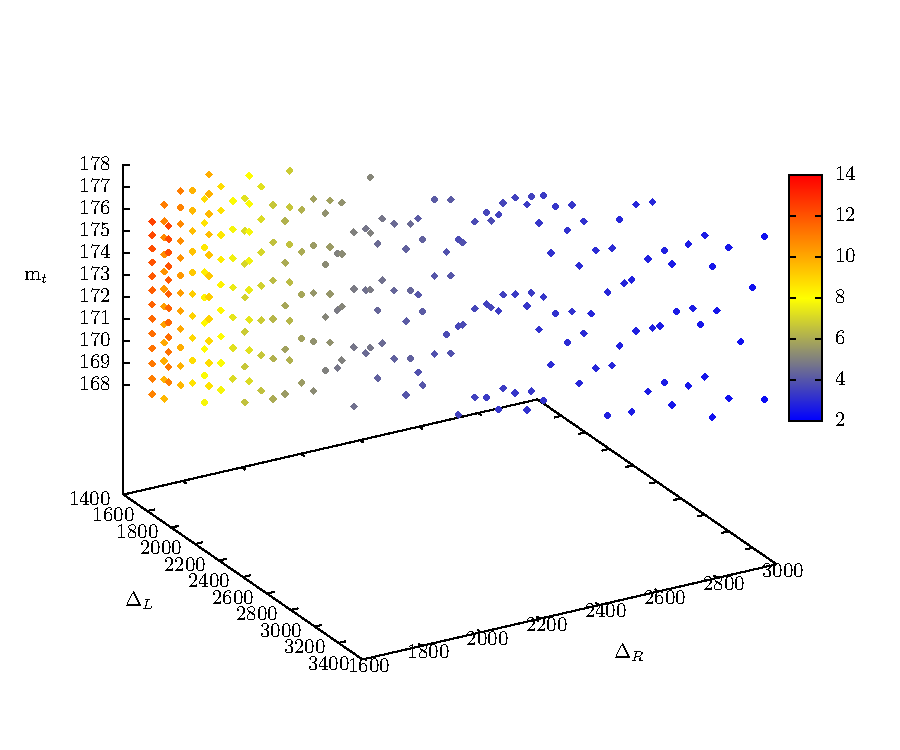
\includegraphics[width=8.5cm,height=7cm]{m3000w5ds100LneRy100dm3000_4d}
	\end{minipage}
	\begin{minipage}[c][10cm][t]{.5\textwidth}
		\vspace*{\fill}
		\centering
		\includegraphics[width=5.5cm,height=5cm]{m3000w5ds100LneRy100dm3000_eigen}
		\includegraphics[width=5cm,height=5cm]{m3000w5ds100LneRy100dm3000_mixing}
		\end{minipage}
	\caption{The results at \(M_0 = 3\) TeV with \(0.5 \leq \Delta_L/\Delta_R \leq 1.5\)}
	\label{fig:res2}
\end{figure}

\noindent The initial runs were performed at a generous mass scale of \(10\) TeV, where we have added the additional condition of \(\Delta_L = \Delta_R\). Solutions are found, as shown in Fig.~\ref{fig:res1}. The precise number is uninteresting as it is largely dependent on the step size and allowed parameter ranges. Similarly, any underlying structure between \(\Delta_{L,R}\) and \(y\) which looks to be present was not considered in any detail. We see the allowed values of top partner masses ranges from around 10 TeV (the composite mass scale, as expected) to 15 TeV, pushing the limits of the LHC in Run 2. We also see that this energy scale is already characterised by a relatively large mixing angle between composite and elementary states, defined for left and right components respectively as:

\begin{equation}
\label{eq4}
\tan{\phi_L} = \frac{\Delta_L}{M_0} \qquad\text{and}\qquad \tan{\phi_R} = \frac{\Delta_R}{M_0 + yf}.
\end{equation}

\noindent Solutions should become more sparse at lower energies. In Fig.~\ref{fig:res2} we have lowered the energy scale but also relaxed the condition that \(\Delta_L\) and \(\Delta_R\) need be identical in the hope of expanding the parameter space. Indeed we find an ample number of solutions still exist. It should be noted here that although more solutions are present at this scale, this is merely a consequence of the widened \(\Delta\) range. Introducing such a feature is entirely permissible, however there are no underlying motivations to do so. We find that top partner masses in this case are scaled down accordingly and now definitely lie within the reach of LHC. Furthermore, the mixing angles are reduced thus indicating we are `closer' to the SM. \\

\begin{figure}[h]
	\centering
	\includegraphics[scale=0.5]{eigen_all}
	\caption{The lightest and heaviest partners over a range of energy scales.}
	\label{fig:res3}
\end{figure}

\noindent We find further that solutions similar to those shown in Figs.~\ref{fig:res1},~\ref{fig:res2} exist over a range of mass scales, as demonstrated in Fig.~\ref{fig:res3}. The significance of this is two-fold. We see that this model remains valid at almost all energy scales the LHC might hope to reach, however in terms of aiding experimental investigation it offers no further help. To refine the allowed parameter space through theoretical considerations alone is difficult; at this stage there are no arguments to hone the first estimates of the \(y\) and \(\Delta_{L,R}\) ranges given above. As for the mass scale, we can look again to QCD; the pion masses are separated from the next resonances by a factor of around 4. Hence to a first approximation we can expect the other resonances in this new strong sector to obey similar behaviour and manifest themselves around the TeV scale, which is consistent with naturalness arguments. Indeed, we already see a slight fine-tuning present at 10 TeV in the mixing angles in that the spread is considerably less than at 3 TeV. This will become more prominent at even higher energies (say 20 TeV), which is an undesirable feature. \\
\hfill\break
The phenomenology of top partners follows their construction from the language of partial compositeness. Searches are ongoing at the LHC. The latest results put a lower mass bound on heavy vector-like pair produced top quarks ranging between 715 GeV and 950 GeV \cite{atlasExotic}, depending on the decay mode. These limits from Run 1 are already approaching the TeV scale at which we expect new physics to be present, and searches will only be enhanced at the higher energies of Run 2. 

\section{Conclusion}
We have shown that composite Higgs models are a viable successor to the SM which is free from quadratic divergences. When fermionic resonances are considered using partial compositeness, top partner masses are found around the TeV scale. The results shown here are drawn from a minimalistic model of a particular symmetry breaking pattern, yet we can expect similar models from the paradigm of a composite Higgs to exhibit similar results. This means if nature chooses such a path then the LHC should be able to tell, and that's definitely an exciting conclusion.

\section*{References}
\bibliography{tqps}

\end{document}
